
\begin{tikzpicture}
\begin{scope}[yshift=-0.75cm]
  \Text[x=-0.5,fontsize=\Large]{$\{$}
  \Vertex[size=0.5,IdAsLabel,x=0,RGB,color={231,195,138}]{g}
  \Vertex[size=0.5,IdAsLabel,x=1,RGB,color={231,195,138}]{c}
  \Vertex[size=0.5,IdAsLabel,x=2,RGB,color={231,195,138}]{e}
  \Vertex[size=0.5,IdAsLabel,x=3,RGB,color={231,195,138}]{h}
  \Text[x=3.5,fontsize=\Large, anchor=west]{$\}=x_2$}
\end{scope}

% \vspace{1em}

\begin{scope}[yshift=-1.5cm]
  \Text[x=-0.5,fontsize=\Large]{$\{$}
  \Vertex[size=0.5,IdAsLabel,x=0,RGB,color={141,203,160}]{f}
  \Vertex[size=0.5,IdAsLabel,x=1,RGB,color={141,203,160}]{e}
  \Vertex[size=0.5,IdAsLabel,x=2,RGB,color={141,203,160}]{a}
  \Vertex[size=0.5,IdAsLabel,x=3,RGB,color={141,203,160}]{h}
  \Text[x=3.5,fontsize=\Large, anchor=west]{$\}=x_3$}

\end{scope}

% \vspace{1em}

\begin{scope}[yshift=-2.25cm]
  \Text[x=-0.5,fontsize=\Large]{$\{$}
  \Vertex[size=0.5,IdAsLabel,x=0,RGB,color={252,98,141}]{i}
  \Vertex[size=0.5,IdAsLabel,x=1,RGB,color={252,98,141}]{j}
  \Vertex[size=0.5,IdAsLabel,x=2,RGB,color={252,98,141}]{f}
  \Vertex[size=0.5,IdAsLabel,x=3,RGB,color={252,98,141}]{b}
  \Text[x=3.5,fontsize=\Large, anchor=west]{$\}=x_4$}
\end{scope}

\begin{scope}
  \Text[x=-0.5,fontsize=\Large]{$\{$}
  \Vertex[size=0.5,IdAsLabel,x=0.5,RGB,color={171,215,230}]{d}
  \Vertex[size=0.5,IdAsLabel,x=1.5,RGB,color={171,215,230}]{h}
  \Vertex[size=0.5,IdAsLabel,x=2.5,RGB,color={171,215,230}]{e}
  \Text[x=3.5,fontsize=\Large, anchor=west]{$\}=x_1$}
\end{scope}
\end{tikzpicture}
